\documentclass{article}

\usepackage{arxiv}

\usepackage[utf8]{inputenc} % allow utf-8 input
\usepackage[T1]{fontenc}    % use 8-bit T1 fonts
\usepackage{lmodern}        % https://github.com/rstudio/rticles/issues/343
\usepackage{hyperref}       % hyperlinks
\usepackage{url}            % simple URL typesetting
\usepackage{booktabs}       % professional-quality tables
\usepackage{amsfonts}       % blackboard math symbols
\usepackage{nicefrac}       % compact symbols for 1/2, etc.
\usepackage{microtype}      % microtypography
\usepackage{lipsum}
\usepackage{graphicx}

\title{Hiking with Tobler: Tracking Movement and Calibrating a Cost
Function for Personalized 3D Accessibility}

\author{
    Christopher D. Higgins
   \\
    Department of Human Geography \\
    University of Toronto Scarborough \\
  1265 Military Trail, Toronto, ON. Canada, M1C 1A4 \\
  \texttt{\href{mailto:cd.higgins@utoronto.ca}{\nolinkurl{cd.higgins@utoronto.ca}}} \\
  }


% Pandoc citation processing
\newlength{\csllabelwidth}
\setlength{\csllabelwidth}{3em}
\newlength{\cslhangindent}
\setlength{\cslhangindent}{1.5em}
% for Pandoc 2.8 to 2.10.1
\newenvironment{cslreferences}%
  {}%
  {\par}
% For Pandoc 2.11+
\newenvironment{CSLReferences}[2] % #1 hanging-ident, #2 entry spacing
 {% don't indent paragraphs
  \setlength{\parindent}{0pt}
  % turn on hanging indent if param 1 is 1
  \ifodd #1 \everypar{\setlength{\hangindent}{\cslhangindent}}\ignorespaces\fi
  % set entry spacing
  \ifnum #2 > 0
  \setlength{\parskip}{#2\baselineskip}
  \fi
 }%
 {}
\usepackage{calc} % for calculating minipage widths
\newcommand{\CSLBlock}[1]{#1\hfill\break}
\newcommand{\CSLLeftMargin}[1]{\parbox[t]{\csllabelwidth}{#1}}
\newcommand{\CSLRightInline}[1]{\parbox[t]{\linewidth - \csllabelwidth}{#1}\break}
\newcommand{\CSLIndent}[1]{\hspace{\cslhangindent}#1}

\usepackage{float}
\usepackage{array}
\usepackage{caption}
\usepackage{graphicx}
\usepackage{siunitx}
\usepackage[normalem]{ulem}
\usepackage{colortbl}
\usepackage{multirow}
\usepackage{hhline}
\usepackage{calc}
\usepackage{tabularx}
\usepackage{threeparttable}
\usepackage{wrapfig}
\usepackage{adjustbox}
\usepackage{hyperref}


\begin{document}
\maketitle

\def\tightlist{}


\begin{abstract}
This paper analyzes the author's travel trajectories to calibrate a
bespoke walking cost function based on Tobler's Hiking Function (THF)
and uses it to estimate personalized accessibility on a 3D network in
Hong Kong. Compared to the THF, the calibrated cost function reflects
slower walking speeds on flatter ground and higher speeds on more sloped
terrain. This latter effect is likely due to the presence of staircases
that enable increased walking speeds on steeper slopes. Accessibility
results using the calibrated function are slightly lower than those from
the THF and highlight the importance of slope-aware cost functions in
modelling walkability.
\end{abstract}

\keywords{
    hiking function
   \and
    route choice
   \and
    trajectory analysis
   \and
    fitness tracker
   \and
    accessibility analysis
  }

\hypertarget{questions}{%
\section{QUESTIONS}\label{questions}}

Hong Kong is an intensely three-dimensional city, not only in terms of
its complex `volumetric' built environment (Bruyns, Higgins, and Nel
2020) but also its mountainous terrain. While working at the Hong Kong
Polytechnic University, I took up hiking on the city's extensive trail
network. But as a quantitative geographer with a general interest in the
potential of sensors for personalized urban data analysis, I could not
help but to combine work and leisure activities and utilized my mobile
phone and smartwatch to capture data on my physical performance. On a
personal level, I became interested in how closely my captured travel
trajectories align with the speeds predicted by Tobler's (1993) `hiking
function.'

On the professional side, I am also broadly interested in the use of
cost functions for accessibility analysis. Modelling pedestrian
accessibility on a 3D network requires the use of an anisotropic cost
function and while Tobler's Hiking Function (THF) has a long history of
applications in the field of archaeology, Goodchild (2020) comments on
the increasing usefulness of hiking functions in a variety of topic
areas in geographical analysis (and includes an early graph of this
paper's data). Indeed, the THF is increasingly utilized as a cost
function in 3D surface (e.g.~water access in Páez et al. (2020)) and
linear network (e.g.~access to rapid transit stations in Higgins (2019))
analysis. Other researchers have used new sources of activity data to
calibrate different cost functions (Brundson 2018; Campbell et al. 2019;
Irmischer and Clarke 2017; Pingel 2010). Some type of hiking function
also appears to underpin routing suggestions on sloped terrain in Google
Maps (Goodchild 2020).

However, the original THF was calibrated to coarse isoline data from
Imhof (1950) and while its predicted speeds may be suitable for
modelling movement on unimproved terrain, it is not clear how well its
predictions extend to walking in an urban 3D network context.
Alternative cost functions could be calibrated for urban walking
specifically, but obtaining accurate GPS trajectories is challenging in
``urban canyon'' contexts like Hong Kong (Ji et al. 2010). In response,
this research utilizes trajectory data captured on trails that exhibit
terrain types similar to what would be found in more urban walking
environments to calibrate a bespoke cost function. I then use the
function to estimate personalized accessibility to an urban amenity on a
3D network.

\hypertarget{methods}{%
\section{METHODS}\label{methods}}

I collected trajectory data over 4 hikes on the trails around Lung Fu
Shan peak and the Pinewood Battery behind the University of Hong Kong in
Central and Western District in 2018. The trails themselves feature dirt
footpaths, segments finished with stone/concrete pavers and pavement,
and stairs at the steepest sections, making them a useful proxy for more
urban walking. Data were collected using an Apple iPhone 8 and Apple
Watch Series 1 through the `Outdoor Walk' tracking in the Fitness
application. This device combination captures latitude and longitude
positioning using the iPhone's GPS receiver, height from sea level using
the barometer (precision of 0.1m), and heart rate readings using from
Apple Watch. The phone applies some smoothing algorithm to the GPS data
and can also use the accelerometer and gyroscope in the watch to augment
positional accuracy in areas with poor or no GPS signal, although these
features are opaque to the user. Readings were captured from the sensors
at 1-second intervals. The resulting workouts were exported as
\texttt{.gpx} files using the Run Gap app for iOS. The trajectories were
cleaned to remove the beginning of the walk to the trail (where the
accuracy of GPS readings is compromised by tall buildings) and a handful
of stops to rest during the hikes. Figure 1 shows the trajectories and a
combined terrain and elevation profile for one of the hikes.

\begin{figure}
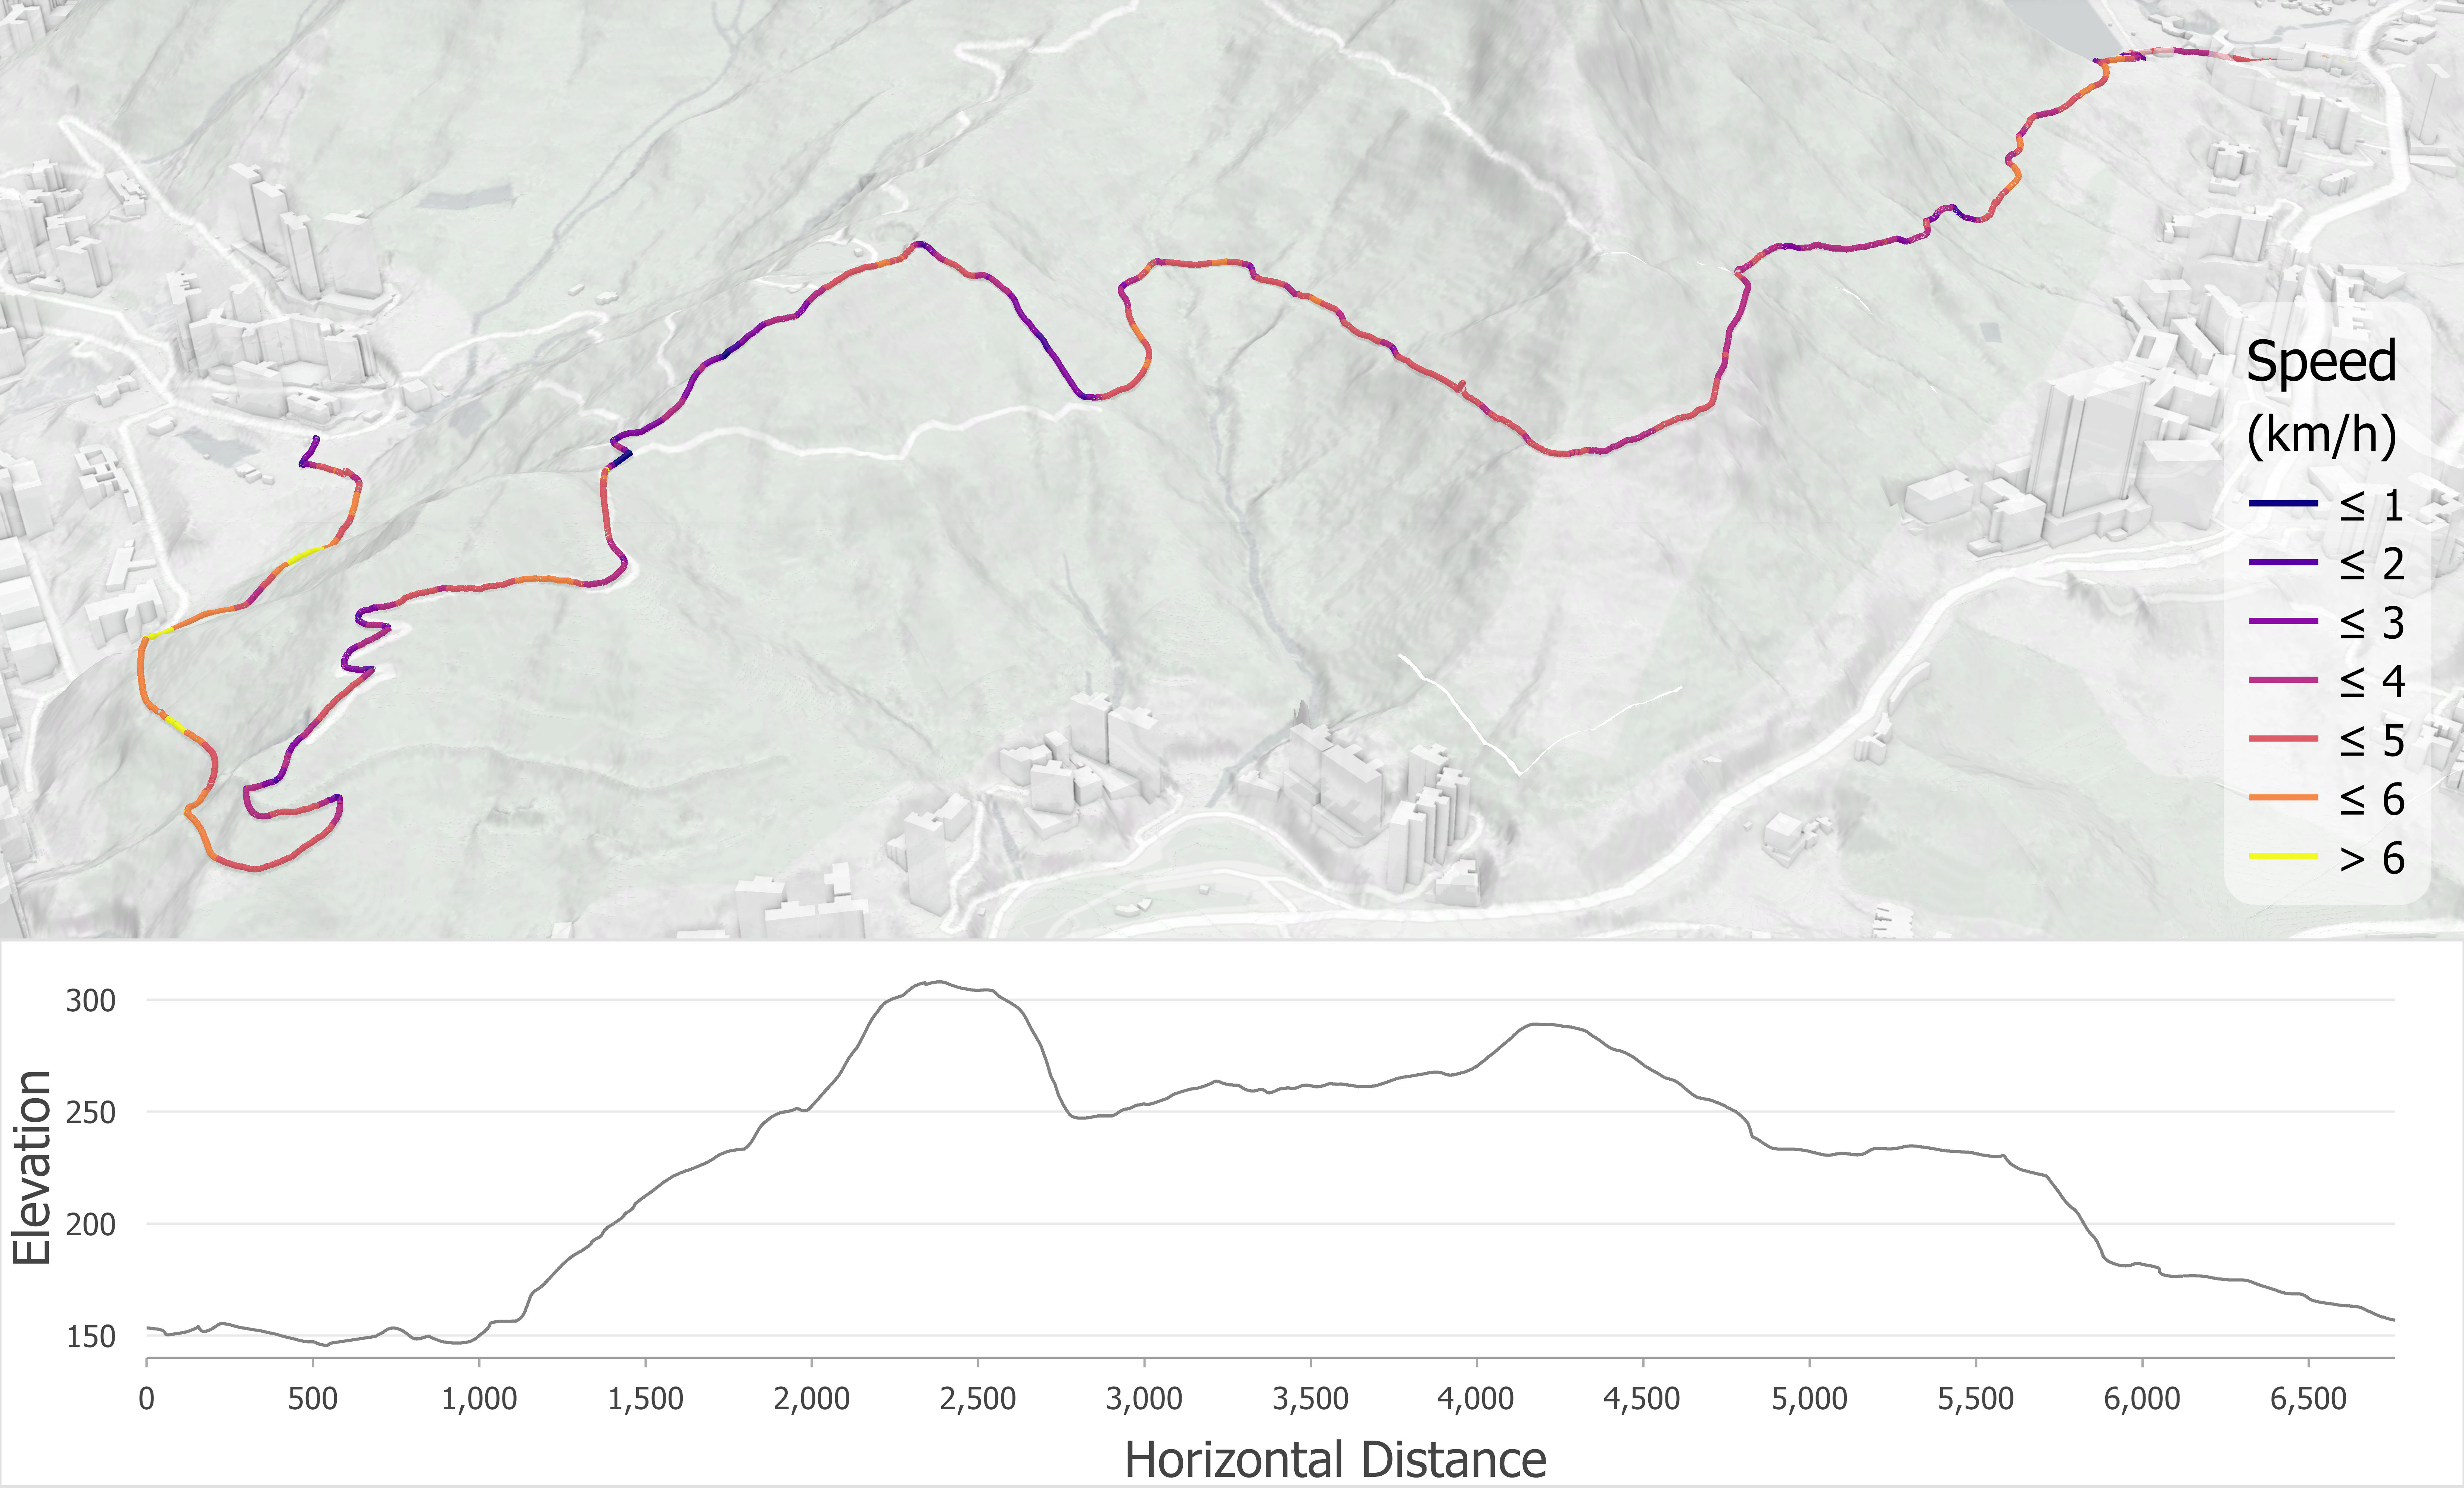
\includegraphics[width=1\linewidth]{./img/Fig_1} \caption{April 29 Hike Trajectory and Profile}\label{fig:fig 1}
\end{figure}

To model travel speeds, Tobler's (1993) hiking function uses an
exponential function to estimate the connection between velocity and
slope:

\[
v = \alpha * e^{(-\beta_1 |g + \beta_2|)}
\]

Where \(v\) is walking velocity in km/h, \(\alpha\) is a constant that
controls the maximum velocity, \(g\) is the gradient of the terrain
measured as the tangent of the angle of the slope in the direction of
travel, \(\beta_1\) controls the rate of decline as the gradient
increases, and \(\beta_2\) offsets the gradient by some amount to
capture how walking speeds are highest on a slight downward gradient. In
Tobler's original formulation, \(\alpha = 6 kph\), \(\beta_1 = 3.5\),
and \(\beta_2 = 0.05\) so that the maximum walking velocity of 6 km/h is
achieved at a gradient of -5\%. I use nonlinear least squares to fit the
generalized hiking function to the trajectory data and compare my walk
speeds with that predicted by Tobler's formulation. To test the
sensitivity of the estimated results to the temporal scale of the
trajectory data, I employed two aggregation strategies including
collapsing the trajectories into 3s, 5s, and 10s time intervals and
calculating average speeds at 1\% gradient intervals.

For the accessibility analysis, a 3D pedestrian network (LandsD 2021;
Sun, Webster, and Zhang 2019) is prepared in a similar manner to that
outlined in Higgins (2019), including splitting links into 10m or less
segments to improve the accuracy of slope-based travel times and
specifying anisotropic travel costs. For simplicity, the travel speed of
any mechanized links (e.g.~travelator, elevator) is set to 2km/h and the
maximum gradient is capped at \(\pm{100}\)\%. To estimate the effects of
the bespoke cost function on personalized accessibility analysis, a
simple scenario is crafted wherein I examine the spatial distribution of
buildings within a 15 min walk of the Kinwick Centre. This building
houses a grocery store and gym and is an interesting destination due to
its location in the topographically-rich SoHo neighbourhood about
halfway up the 800m Central-Mid-Levels escalator system. Using ArcGIS
Pro, travel times are calculated three times: using the fit function and
the THF to account for slope and a third time assuming the network is 2D
with a constant walk speed of 5km/h.

\hypertarget{findings}{%
\section{FINDINGS}\label{findings}}

Results of the NLS models are presented in Table 1 and graphed in Figure
2. The sensitivity analysis suggests that the models are reasonably
stable in parameters across all model specifications. The exception is
the \(\beta_2\) offset parameter which is insignificant in all binned
models, indicating the cost curves in this category are estimated to be
symmetric around a 0\% gradient. Recognizing that neither AIC nor BIC
are useful for comparing model fit across different sample sizes, I
focus on the results for the original raw 1s data. Results indicate that
my maximum walking speed of about 4.6km/h occurs on about a -3.3\%
gradient rather than the -5\% in Tobler's formulation. My average
flat-ground walking speed is also a bit slower than what Tobler (1993)
would predict at about 4.4 km/h. On the other hand, I tend to be faster
on higher slopes than predicted by the original THF, likely due to the
prevalence of staircases on the steepest sections of the trail.

 
  \providecommand{\huxb}[2]{\arrayrulecolor[RGB]{#1}\global\arrayrulewidth=#2pt}
  \providecommand{\huxvb}[2]{\color[RGB]{#1}\vrule width #2pt}
  \providecommand{\huxtpad}[1]{\rule{0pt}{#1}}
  \providecommand{\huxbpad}[1]{\rule[-#1]{0pt}{#1}}

\begin{table}[ht]
\begin{centerbox}
\begin{threeparttable}
\captionsetup{justification=centering,singlelinecheck=off}
\caption{Table 1. NLS Model Results}
 \label{tab:table 1}
\setlength{\tabcolsep}{0pt}
\begin{tabularx}{1\textwidth}{p{0.111111111111111\textwidth} p{0.111111111111111\textwidth} p{0.111111111111111\textwidth} p{0.111111111111111\textwidth} p{0.111111111111111\textwidth} p{0.111111111111111\textwidth} p{0.111111111111111\textwidth} p{0.111111111111111\textwidth} p{0.111111111111111\textwidth}}


\hhline{>{\huxb{0, 0, 0}{0.8}}->{\huxb{0, 0, 0}{0.8}}->{\huxb{0, 0, 0}{0.8}}->{\huxb{0, 0, 0}{0.8}}->{\huxb{0, 0, 0}{0.8}}->{\huxb{0, 0, 0}{0.8}}->{\huxb{0, 0, 0}{0.8}}->{\huxb{0, 0, 0}{0.8}}->{\huxb{0, 0, 0}{0.8}}-}
\arrayrulecolor{black}

\multicolumn{1}{!{\huxvb{0, 0, 0}{0}}p{0.111111111111111\textwidth}!{\huxvb{0, 0, 0}{0}}}{\hspace{6pt}\parbox[b]{0.111111111111111\textwidth-6pt-6pt}{\huxtpad{6pt + 1em}\centering \huxbpad{6pt}}} &
\multicolumn{1}{p{0.111111111111111\textwidth}!{\huxvb{0, 0, 0}{0}}}{\hspace{6pt}\parbox[b]{0.111111111111111\textwidth-6pt-6pt}{\huxtpad{6pt + 1em}\centering 1s\_raw\huxbpad{6pt}}} &
\multicolumn{1}{p{0.111111111111111\textwidth}!{\huxvb{0, 0, 0}{0}}}{\hspace{6pt}\parbox[b]{0.111111111111111\textwidth-6pt-6pt}{\huxtpad{6pt + 1em}\centering 3s\_agg\huxbpad{6pt}}} &
\multicolumn{1}{p{0.111111111111111\textwidth}!{\huxvb{0, 0, 0}{0}}}{\hspace{6pt}\parbox[b]{0.111111111111111\textwidth-6pt-6pt}{\huxtpad{6pt + 1em}\centering 5s\_agg\huxbpad{6pt}}} &
\multicolumn{1}{p{0.111111111111111\textwidth}!{\huxvb{0, 0, 0}{0}}}{\hspace{6pt}\parbox[b]{0.111111111111111\textwidth-6pt-6pt}{\huxtpad{6pt + 1em}\centering 10s\_agg\huxbpad{6pt}}} &
\multicolumn{1}{p{0.111111111111111\textwidth}!{\huxvb{0, 0, 0}{0}}}{\hspace{6pt}\parbox[b]{0.111111111111111\textwidth-6pt-6pt}{\huxtpad{6pt + 1em}\centering 1s\_bin\huxbpad{6pt}}} &
\multicolumn{1}{p{0.111111111111111\textwidth}!{\huxvb{0, 0, 0}{0}}}{\hspace{6pt}\parbox[b]{0.111111111111111\textwidth-6pt-6pt}{\huxtpad{6pt + 1em}\centering 3s\_bin\huxbpad{6pt}}} &
\multicolumn{1}{p{0.111111111111111\textwidth}!{\huxvb{0, 0, 0}{0}}}{\hspace{6pt}\parbox[b]{0.111111111111111\textwidth-6pt-6pt}{\huxtpad{6pt + 1em}\centering 5s\_bin\huxbpad{6pt}}} &
\multicolumn{1}{p{0.111111111111111\textwidth}!{\huxvb{0, 0, 0}{0}}}{\hspace{6pt}\parbox[b]{0.111111111111111\textwidth-6pt-6pt}{\huxtpad{6pt + 1em}\centering 10s\_bin\huxbpad{6pt}}} \tabularnewline[-0.5pt]


\hhline{>{\huxb{255, 255, 255}{0.4}}->{\huxb{0, 0, 0}{0.4}}->{\huxb{0, 0, 0}{0.4}}->{\huxb{0, 0, 0}{0.4}}->{\huxb{0, 0, 0}{0.4}}->{\huxb{0, 0, 0}{0.4}}->{\huxb{0, 0, 0}{0.4}}->{\huxb{0, 0, 0}{0.4}}->{\huxb{0, 0, 0}{0.4}}-}
\arrayrulecolor{black}

\multicolumn{1}{!{\huxvb{0, 0, 0}{0}}p{0.111111111111111\textwidth}!{\huxvb{0, 0, 0}{0}}}{\hspace{6pt}\parbox[b]{0.111111111111111\textwidth-6pt-6pt}{\huxtpad{6pt + 1em}\raggedright a\huxbpad{6pt}}} &
\multicolumn{1}{p{0.111111111111111\textwidth}!{\huxvb{0, 0, 0}{0}}}{\hspace{6pt}\parbox[b]{0.111111111111111\textwidth-6pt-6pt}{\huxtpad{6pt + 1em}\raggedleft 4.607 ***\huxbpad{6pt}}} &
\multicolumn{1}{p{0.111111111111111\textwidth}!{\huxvb{0, 0, 0}{0}}}{\hspace{6pt}\parbox[b]{0.111111111111111\textwidth-6pt-6pt}{\huxtpad{6pt + 1em}\raggedleft 4.643 ***\huxbpad{6pt}}} &
\multicolumn{1}{p{0.111111111111111\textwidth}!{\huxvb{0, 0, 0}{0}}}{\hspace{6pt}\parbox[b]{0.111111111111111\textwidth-6pt-6pt}{\huxtpad{6pt + 1em}\raggedleft 4.636 ***\huxbpad{6pt}}} &
\multicolumn{1}{p{0.111111111111111\textwidth}!{\huxvb{0, 0, 0}{0}}}{\hspace{6pt}\parbox[b]{0.111111111111111\textwidth-6pt-6pt}{\huxtpad{6pt + 1em}\raggedleft 4.637 ***\huxbpad{6pt}}} &
\multicolumn{1}{p{0.111111111111111\textwidth}!{\huxvb{0, 0, 0}{0}}}{\hspace{6pt}\parbox[b]{0.111111111111111\textwidth-6pt-6pt}{\huxtpad{6pt + 1em}\raggedleft 4.897 ***\huxbpad{6pt}}} &
\multicolumn{1}{p{0.111111111111111\textwidth}!{\huxvb{0, 0, 0}{0}}}{\hspace{6pt}\parbox[b]{0.111111111111111\textwidth-6pt-6pt}{\huxtpad{6pt + 1em}\raggedleft 4.599 ***\huxbpad{6pt}}} &
\multicolumn{1}{p{0.111111111111111\textwidth}!{\huxvb{0, 0, 0}{0}}}{\hspace{6pt}\parbox[b]{0.111111111111111\textwidth-6pt-6pt}{\huxtpad{6pt + 1em}\raggedleft 4.650 ***\huxbpad{6pt}}} &
\multicolumn{1}{p{0.111111111111111\textwidth}!{\huxvb{0, 0, 0}{0}}}{\hspace{6pt}\parbox[b]{0.111111111111111\textwidth-6pt-6pt}{\huxtpad{6pt + 1em}\raggedleft 4.610 ***\huxbpad{6pt}}} \tabularnewline[-0.5pt]


\hhline{}
\arrayrulecolor{black}

\multicolumn{1}{!{\huxvb{0, 0, 0}{0}}p{0.111111111111111\textwidth}!{\huxvb{0, 0, 0}{0}}}{\hspace{6pt}\parbox[b]{0.111111111111111\textwidth-6pt-6pt}{\huxtpad{6pt + 1em}\raggedright \huxbpad{6pt}}} &
\multicolumn{1}{p{0.111111111111111\textwidth}!{\huxvb{0, 0, 0}{0}}}{\hspace{6pt}\parbox[b]{0.111111111111111\textwidth-6pt-6pt}{\huxtpad{6pt + 1em}\raggedleft (0.014)\hphantom{0}\hphantom{0}\hphantom{0}\huxbpad{6pt}}} &
\multicolumn{1}{p{0.111111111111111\textwidth}!{\huxvb{0, 0, 0}{0}}}{\hspace{6pt}\parbox[b]{0.111111111111111\textwidth-6pt-6pt}{\huxtpad{6pt + 1em}\raggedleft (0.021)\hphantom{0}\hphantom{0}\hphantom{0}\huxbpad{6pt}}} &
\multicolumn{1}{p{0.111111111111111\textwidth}!{\huxvb{0, 0, 0}{0}}}{\hspace{6pt}\parbox[b]{0.111111111111111\textwidth-6pt-6pt}{\huxtpad{6pt + 1em}\raggedleft (0.027)\hphantom{0}\hphantom{0}\hphantom{0}\huxbpad{6pt}}} &
\multicolumn{1}{p{0.111111111111111\textwidth}!{\huxvb{0, 0, 0}{0}}}{\hspace{6pt}\parbox[b]{0.111111111111111\textwidth-6pt-6pt}{\huxtpad{6pt + 1em}\raggedleft (0.038)\hphantom{0}\hphantom{0}\hphantom{0}\huxbpad{6pt}}} &
\multicolumn{1}{p{0.111111111111111\textwidth}!{\huxvb{0, 0, 0}{0}}}{\hspace{6pt}\parbox[b]{0.111111111111111\textwidth-6pt-6pt}{\huxtpad{6pt + 1em}\raggedleft (0.120)\hphantom{0}\hphantom{0}\hphantom{0}\huxbpad{6pt}}} &
\multicolumn{1}{p{0.111111111111111\textwidth}!{\huxvb{0, 0, 0}{0}}}{\hspace{6pt}\parbox[b]{0.111111111111111\textwidth-6pt-6pt}{\huxtpad{6pt + 1em}\raggedleft (0.064)\hphantom{0}\hphantom{0}\hphantom{0}\huxbpad{6pt}}} &
\multicolumn{1}{p{0.111111111111111\textwidth}!{\huxvb{0, 0, 0}{0}}}{\hspace{6pt}\parbox[b]{0.111111111111111\textwidth-6pt-6pt}{\huxtpad{6pt + 1em}\raggedleft (0.068)\hphantom{0}\hphantom{0}\hphantom{0}\huxbpad{6pt}}} &
\multicolumn{1}{p{0.111111111111111\textwidth}!{\huxvb{0, 0, 0}{0}}}{\hspace{6pt}\parbox[b]{0.111111111111111\textwidth-6pt-6pt}{\huxtpad{6pt + 1em}\raggedleft (0.071)\hphantom{0}\hphantom{0}\hphantom{0}\huxbpad{6pt}}} \tabularnewline[-0.5pt]


\hhline{}
\arrayrulecolor{black}

\multicolumn{1}{!{\huxvb{0, 0, 0}{0}}p{0.111111111111111\textwidth}!{\huxvb{0, 0, 0}{0}}}{\hspace{6pt}\parbox[b]{0.111111111111111\textwidth-6pt-6pt}{\huxtpad{6pt + 1em}\raggedright b1\huxbpad{6pt}}} &
\multicolumn{1}{p{0.111111111111111\textwidth}!{\huxvb{0, 0, 0}{0}}}{\hspace{6pt}\parbox[b]{0.111111111111111\textwidth-6pt-6pt}{\huxtpad{6pt + 1em}\raggedleft 1.542 ***\huxbpad{6pt}}} &
\multicolumn{1}{p{0.111111111111111\textwidth}!{\huxvb{0, 0, 0}{0}}}{\hspace{6pt}\parbox[b]{0.111111111111111\textwidth-6pt-6pt}{\huxtpad{6pt + 1em}\raggedleft 1.694 ***\huxbpad{6pt}}} &
\multicolumn{1}{p{0.111111111111111\textwidth}!{\huxvb{0, 0, 0}{0}}}{\hspace{6pt}\parbox[b]{0.111111111111111\textwidth-6pt-6pt}{\huxtpad{6pt + 1em}\raggedleft 1.696 ***\huxbpad{6pt}}} &
\multicolumn{1}{p{0.111111111111111\textwidth}!{\huxvb{0, 0, 0}{0}}}{\hspace{6pt}\parbox[b]{0.111111111111111\textwidth-6pt-6pt}{\huxtpad{6pt + 1em}\raggedleft 1.723 ***\huxbpad{6pt}}} &
\multicolumn{1}{p{0.111111111111111\textwidth}!{\huxvb{0, 0, 0}{0}}}{\hspace{6pt}\parbox[b]{0.111111111111111\textwidth-6pt-6pt}{\huxtpad{6pt + 1em}\raggedleft 1.639 ***\huxbpad{6pt}}} &
\multicolumn{1}{p{0.111111111111111\textwidth}!{\huxvb{0, 0, 0}{0}}}{\hspace{6pt}\parbox[b]{0.111111111111111\textwidth-6pt-6pt}{\huxtpad{6pt + 1em}\raggedleft 1.615 ***\huxbpad{6pt}}} &
\multicolumn{1}{p{0.111111111111111\textwidth}!{\huxvb{0, 0, 0}{0}}}{\hspace{6pt}\parbox[b]{0.111111111111111\textwidth-6pt-6pt}{\huxtpad{6pt + 1em}\raggedleft 1.696 ***\huxbpad{6pt}}} &
\multicolumn{1}{p{0.111111111111111\textwidth}!{\huxvb{0, 0, 0}{0}}}{\hspace{6pt}\parbox[b]{0.111111111111111\textwidth-6pt-6pt}{\huxtpad{6pt + 1em}\raggedleft 1.699 ***\huxbpad{6pt}}} \tabularnewline[-0.5pt]


\hhline{}
\arrayrulecolor{black}

\multicolumn{1}{!{\huxvb{0, 0, 0}{0}}p{0.111111111111111\textwidth}!{\huxvb{0, 0, 0}{0}}}{\hspace{6pt}\parbox[b]{0.111111111111111\textwidth-6pt-6pt}{\huxtpad{6pt + 1em}\raggedright \huxbpad{6pt}}} &
\multicolumn{1}{p{0.111111111111111\textwidth}!{\huxvb{0, 0, 0}{0}}}{\hspace{6pt}\parbox[b]{0.111111111111111\textwidth-6pt-6pt}{\huxtpad{6pt + 1em}\raggedleft (0.019)\hphantom{0}\hphantom{0}\hphantom{0}\huxbpad{6pt}}} &
\multicolumn{1}{p{0.111111111111111\textwidth}!{\huxvb{0, 0, 0}{0}}}{\hspace{6pt}\parbox[b]{0.111111111111111\textwidth-6pt-6pt}{\huxtpad{6pt + 1em}\raggedleft (0.032)\hphantom{0}\hphantom{0}\hphantom{0}\huxbpad{6pt}}} &
\multicolumn{1}{p{0.111111111111111\textwidth}!{\huxvb{0, 0, 0}{0}}}{\hspace{6pt}\parbox[b]{0.111111111111111\textwidth-6pt-6pt}{\huxtpad{6pt + 1em}\raggedleft (0.041)\hphantom{0}\hphantom{0}\hphantom{0}\huxbpad{6pt}}} &
\multicolumn{1}{p{0.111111111111111\textwidth}!{\huxvb{0, 0, 0}{0}}}{\hspace{6pt}\parbox[b]{0.111111111111111\textwidth-6pt-6pt}{\huxtpad{6pt + 1em}\raggedleft (0.058)\hphantom{0}\hphantom{0}\hphantom{0}\huxbpad{6pt}}} &
\multicolumn{1}{p{0.111111111111111\textwidth}!{\huxvb{0, 0, 0}{0}}}{\hspace{6pt}\parbox[b]{0.111111111111111\textwidth-6pt-6pt}{\huxtpad{6pt + 1em}\raggedleft (0.069)\hphantom{0}\hphantom{0}\hphantom{0}\huxbpad{6pt}}} &
\multicolumn{1}{p{0.111111111111111\textwidth}!{\huxvb{0, 0, 0}{0}}}{\hspace{6pt}\parbox[b]{0.111111111111111\textwidth-6pt-6pt}{\huxtpad{6pt + 1em}\raggedleft (0.045)\hphantom{0}\hphantom{0}\hphantom{0}\huxbpad{6pt}}} &
\multicolumn{1}{p{0.111111111111111\textwidth}!{\huxvb{0, 0, 0}{0}}}{\hspace{6pt}\parbox[b]{0.111111111111111\textwidth-6pt-6pt}{\huxtpad{6pt + 1em}\raggedleft (0.052)\hphantom{0}\hphantom{0}\hphantom{0}\huxbpad{6pt}}} &
\multicolumn{1}{p{0.111111111111111\textwidth}!{\huxvb{0, 0, 0}{0}}}{\hspace{6pt}\parbox[b]{0.111111111111111\textwidth-6pt-6pt}{\huxtpad{6pt + 1em}\raggedleft (0.059)\hphantom{0}\hphantom{0}\hphantom{0}\huxbpad{6pt}}} \tabularnewline[-0.5pt]


\hhline{}
\arrayrulecolor{black}

\multicolumn{1}{!{\huxvb{0, 0, 0}{0}}p{0.111111111111111\textwidth}!{\huxvb{0, 0, 0}{0}}}{\hspace{6pt}\parbox[b]{0.111111111111111\textwidth-6pt-6pt}{\huxtpad{6pt + 1em}\raggedright b2\huxbpad{6pt}}} &
\multicolumn{1}{p{0.111111111111111\textwidth}!{\huxvb{0, 0, 0}{0}}}{\hspace{6pt}\parbox[b]{0.111111111111111\textwidth-6pt-6pt}{\huxtpad{6pt + 1em}\raggedleft 0.033 ***\huxbpad{6pt}}} &
\multicolumn{1}{p{0.111111111111111\textwidth}!{\huxvb{0, 0, 0}{0}}}{\hspace{6pt}\parbox[b]{0.111111111111111\textwidth-6pt-6pt}{\huxtpad{6pt + 1em}\raggedleft 0.017 ***\huxbpad{6pt}}} &
\multicolumn{1}{p{0.111111111111111\textwidth}!{\huxvb{0, 0, 0}{0}}}{\hspace{6pt}\parbox[b]{0.111111111111111\textwidth-6pt-6pt}{\huxtpad{6pt + 1em}\raggedleft 0.013 ***\huxbpad{6pt}}} &
\multicolumn{1}{p{0.111111111111111\textwidth}!{\huxvb{0, 0, 0}{0}}}{\hspace{6pt}\parbox[b]{0.111111111111111\textwidth-6pt-6pt}{\huxtpad{6pt + 1em}\raggedleft 0.014 ***\huxbpad{6pt}}} &
\multicolumn{1}{p{0.111111111111111\textwidth}!{\huxvb{0, 0, 0}{0}}}{\hspace{6pt}\parbox[b]{0.111111111111111\textwidth-6pt-6pt}{\huxtpad{6pt + 1em}\raggedleft -0.011\hphantom{0}\hphantom{0}\hphantom{0}\hphantom{0}\huxbpad{6pt}}} &
\multicolumn{1}{p{0.111111111111111\textwidth}!{\huxvb{0, 0, 0}{0}}}{\hspace{6pt}\parbox[b]{0.111111111111111\textwidth-6pt-6pt}{\huxtpad{6pt + 1em}\raggedleft -0.006\hphantom{0}\hphantom{0}\hphantom{0}\hphantom{0}\huxbpad{6pt}}} &
\multicolumn{1}{p{0.111111111111111\textwidth}!{\huxvb{0, 0, 0}{0}}}{\hspace{6pt}\parbox[b]{0.111111111111111\textwidth-6pt-6pt}{\huxtpad{6pt + 1em}\raggedleft -0.003\hphantom{0}\hphantom{0}\hphantom{0}\hphantom{0}\huxbpad{6pt}}} &
\multicolumn{1}{p{0.111111111111111\textwidth}!{\huxvb{0, 0, 0}{0}}}{\hspace{6pt}\parbox[b]{0.111111111111111\textwidth-6pt-6pt}{\huxtpad{6pt + 1em}\raggedleft 0.004\hphantom{0}\hphantom{0}\hphantom{0}\hphantom{0}\huxbpad{6pt}}} \tabularnewline[-0.5pt]


\hhline{}
\arrayrulecolor{black}

\multicolumn{1}{!{\huxvb{0, 0, 0}{0}}p{0.111111111111111\textwidth}!{\huxvb{0, 0, 0}{0}}}{\hspace{6pt}\parbox[b]{0.111111111111111\textwidth-6pt-6pt}{\huxtpad{6pt + 1em}\raggedright \huxbpad{6pt}}} &
\multicolumn{1}{p{0.111111111111111\textwidth}!{\huxvb{0, 0, 0}{0}}}{\hspace{6pt}\parbox[b]{0.111111111111111\textwidth-6pt-6pt}{\huxtpad{6pt + 1em}\raggedleft (0.001)\hphantom{0}\hphantom{0}\hphantom{0}\huxbpad{6pt}}} &
\multicolumn{1}{p{0.111111111111111\textwidth}!{\huxvb{0, 0, 0}{0}}}{\hspace{6pt}\parbox[b]{0.111111111111111\textwidth-6pt-6pt}{\huxtpad{6pt + 1em}\raggedleft (0.002)\hphantom{0}\hphantom{0}\hphantom{0}\huxbpad{6pt}}} &
\multicolumn{1}{p{0.111111111111111\textwidth}!{\huxvb{0, 0, 0}{0}}}{\hspace{6pt}\parbox[b]{0.111111111111111\textwidth-6pt-6pt}{\huxtpad{6pt + 1em}\raggedleft (0.002)\hphantom{0}\hphantom{0}\hphantom{0}\huxbpad{6pt}}} &
\multicolumn{1}{p{0.111111111111111\textwidth}!{\huxvb{0, 0, 0}{0}}}{\hspace{6pt}\parbox[b]{0.111111111111111\textwidth-6pt-6pt}{\huxtpad{6pt + 1em}\raggedleft (0.003)\hphantom{0}\hphantom{0}\hphantom{0}\huxbpad{6pt}}} &
\multicolumn{1}{p{0.111111111111111\textwidth}!{\huxvb{0, 0, 0}{0}}}{\hspace{6pt}\parbox[b]{0.111111111111111\textwidth-6pt-6pt}{\huxtpad{6pt + 1em}\raggedleft (0.009)\hphantom{0}\hphantom{0}\hphantom{0}\huxbpad{6pt}}} &
\multicolumn{1}{p{0.111111111111111\textwidth}!{\huxvb{0, 0, 0}{0}}}{\hspace{6pt}\parbox[b]{0.111111111111111\textwidth-6pt-6pt}{\huxtpad{6pt + 1em}\raggedleft (0.005)\hphantom{0}\hphantom{0}\hphantom{0}\huxbpad{6pt}}} &
\multicolumn{1}{p{0.111111111111111\textwidth}!{\huxvb{0, 0, 0}{0}}}{\hspace{6pt}\parbox[b]{0.111111111111111\textwidth-6pt-6pt}{\huxtpad{6pt + 1em}\raggedleft (0.005)\hphantom{0}\hphantom{0}\hphantom{0}\huxbpad{6pt}}} &
\multicolumn{1}{p{0.111111111111111\textwidth}!{\huxvb{0, 0, 0}{0}}}{\hspace{6pt}\parbox[b]{0.111111111111111\textwidth-6pt-6pt}{\huxtpad{6pt + 1em}\raggedleft (0.006)\hphantom{0}\hphantom{0}\hphantom{0}\huxbpad{6pt}}} \tabularnewline[-0.5pt]


\hhline{>{\huxb{255, 255, 255}{0.4}}->{\huxb{0, 0, 0}{0.4}}->{\huxb{0, 0, 0}{0.4}}->{\huxb{0, 0, 0}{0.4}}->{\huxb{0, 0, 0}{0.4}}->{\huxb{0, 0, 0}{0.4}}->{\huxb{0, 0, 0}{0.4}}->{\huxb{0, 0, 0}{0.4}}->{\huxb{0, 0, 0}{0.4}}-}
\arrayrulecolor{black}

\multicolumn{1}{!{\huxvb{0, 0, 0}{0}}p{0.111111111111111\textwidth}!{\huxvb{0, 0, 0}{0}}}{\hspace{6pt}\parbox[b]{0.111111111111111\textwidth-6pt-6pt}{\huxtpad{6pt + 1em}\raggedright N\huxbpad{6pt}}} &
\multicolumn{1}{p{0.111111111111111\textwidth}!{\huxvb{0, 0, 0}{0}}}{\hspace{6pt}\parbox[b]{0.111111111111111\textwidth-6pt-6pt}{\huxtpad{6pt + 1em}\raggedleft 14449\hphantom{0}\hphantom{0}\hphantom{0}\hphantom{0}\hphantom{0}\hphantom{0}\hphantom{0}\hphantom{0}\huxbpad{6pt}}} &
\multicolumn{1}{p{0.111111111111111\textwidth}!{\huxvb{0, 0, 0}{0}}}{\hspace{6pt}\parbox[b]{0.111111111111111\textwidth-6pt-6pt}{\huxtpad{6pt + 1em}\raggedleft 4810\hphantom{0}\hphantom{0}\hphantom{0}\hphantom{0}\hphantom{0}\hphantom{0}\hphantom{0}\hphantom{0}\huxbpad{6pt}}} &
\multicolumn{1}{p{0.111111111111111\textwidth}!{\huxvb{0, 0, 0}{0}}}{\hspace{6pt}\parbox[b]{0.111111111111111\textwidth-6pt-6pt}{\huxtpad{6pt + 1em}\raggedleft 2881\hphantom{0}\hphantom{0}\hphantom{0}\hphantom{0}\hphantom{0}\hphantom{0}\hphantom{0}\hphantom{0}\huxbpad{6pt}}} &
\multicolumn{1}{p{0.111111111111111\textwidth}!{\huxvb{0, 0, 0}{0}}}{\hspace{6pt}\parbox[b]{0.111111111111111\textwidth-6pt-6pt}{\huxtpad{6pt + 1em}\raggedleft 1436\hphantom{0}\hphantom{0}\hphantom{0}\hphantom{0}\hphantom{0}\hphantom{0}\hphantom{0}\hphantom{0}\huxbpad{6pt}}} &
\multicolumn{1}{p{0.111111111111111\textwidth}!{\huxvb{0, 0, 0}{0}}}{\hspace{6pt}\parbox[b]{0.111111111111111\textwidth-6pt-6pt}{\huxtpad{6pt + 1em}\raggedleft 172\hphantom{0}\hphantom{0}\hphantom{0}\hphantom{0}\hphantom{0}\hphantom{0}\hphantom{0}\hphantom{0}\huxbpad{6pt}}} &
\multicolumn{1}{p{0.111111111111111\textwidth}!{\huxvb{0, 0, 0}{0}}}{\hspace{6pt}\parbox[b]{0.111111111111111\textwidth-6pt-6pt}{\huxtpad{6pt + 1em}\raggedleft 150\hphantom{0}\hphantom{0}\hphantom{0}\hphantom{0}\hphantom{0}\hphantom{0}\hphantom{0}\hphantom{0}\huxbpad{6pt}}} &
\multicolumn{1}{p{0.111111111111111\textwidth}!{\huxvb{0, 0, 0}{0}}}{\hspace{6pt}\parbox[b]{0.111111111111111\textwidth-6pt-6pt}{\huxtpad{6pt + 1em}\raggedleft 137\hphantom{0}\hphantom{0}\hphantom{0}\hphantom{0}\hphantom{0}\hphantom{0}\hphantom{0}\hphantom{0}\huxbpad{6pt}}} &
\multicolumn{1}{p{0.111111111111111\textwidth}!{\huxvb{0, 0, 0}{0}}}{\hspace{6pt}\parbox[b]{0.111111111111111\textwidth-6pt-6pt}{\huxtpad{6pt + 1em}\raggedleft 122\hphantom{0}\hphantom{0}\hphantom{0}\hphantom{0}\hphantom{0}\hphantom{0}\hphantom{0}\hphantom{0}\huxbpad{6pt}}} \tabularnewline[-0.5pt]


\hhline{}
\arrayrulecolor{black}

\multicolumn{1}{!{\huxvb{0, 0, 0}{0}}p{0.111111111111111\textwidth}!{\huxvb{0, 0, 0}{0}}}{\hspace{6pt}\parbox[b]{0.111111111111111\textwidth-6pt-6pt}{\huxtpad{6pt + 1em}\raggedright AIC\huxbpad{6pt}}} &
\multicolumn{1}{p{0.111111111111111\textwidth}!{\huxvb{0, 0, 0}{0}}}{\hspace{6pt}\parbox[b]{0.111111111111111\textwidth-6pt-6pt}{\huxtpad{6pt + 1em}\raggedleft 37617.827\hphantom{0}\hphantom{0}\hphantom{0}\hphantom{0}\huxbpad{6pt}}} &
\multicolumn{1}{p{0.111111111111111\textwidth}!{\huxvb{0, 0, 0}{0}}}{\hspace{6pt}\parbox[b]{0.111111111111111\textwidth-6pt-6pt}{\huxtpad{6pt + 1em}\raggedleft 11938.276\hphantom{0}\hphantom{0}\hphantom{0}\hphantom{0}\huxbpad{6pt}}} &
\multicolumn{1}{p{0.111111111111111\textwidth}!{\huxvb{0, 0, 0}{0}}}{\hspace{6pt}\parbox[b]{0.111111111111111\textwidth-6pt-6pt}{\huxtpad{6pt + 1em}\raggedleft 7093.872\hphantom{0}\hphantom{0}\hphantom{0}\hphantom{0}\huxbpad{6pt}}} &
\multicolumn{1}{p{0.111111111111111\textwidth}!{\huxvb{0, 0, 0}{0}}}{\hspace{6pt}\parbox[b]{0.111111111111111\textwidth-6pt-6pt}{\huxtpad{6pt + 1em}\raggedleft 3488.195\hphantom{0}\hphantom{0}\hphantom{0}\hphantom{0}\huxbpad{6pt}}} &
\multicolumn{1}{p{0.111111111111111\textwidth}!{\huxvb{0, 0, 0}{0}}}{\hspace{6pt}\parbox[b]{0.111111111111111\textwidth-6pt-6pt}{\huxtpad{6pt + 1em}\raggedleft 256.195\hphantom{0}\hphantom{0}\hphantom{0}\hphantom{0}\huxbpad{6pt}}} &
\multicolumn{1}{p{0.111111111111111\textwidth}!{\huxvb{0, 0, 0}{0}}}{\hspace{6pt}\parbox[b]{0.111111111111111\textwidth-6pt-6pt}{\huxtpad{6pt + 1em}\raggedleft 61.704\hphantom{0}\hphantom{0}\hphantom{0}\hphantom{0}\huxbpad{6pt}}} &
\multicolumn{1}{p{0.111111111111111\textwidth}!{\huxvb{0, 0, 0}{0}}}{\hspace{6pt}\parbox[b]{0.111111111111111\textwidth-6pt-6pt}{\huxtpad{6pt + 1em}\raggedleft 75.518\hphantom{0}\hphantom{0}\hphantom{0}\hphantom{0}\huxbpad{6pt}}} &
\multicolumn{1}{p{0.111111111111111\textwidth}!{\huxvb{0, 0, 0}{0}}}{\hspace{6pt}\parbox[b]{0.111111111111111\textwidth-6pt-6pt}{\huxtpad{6pt + 1em}\raggedleft 69.701\hphantom{0}\hphantom{0}\hphantom{0}\hphantom{0}\huxbpad{6pt}}} \tabularnewline[-0.5pt]


\hhline{}
\arrayrulecolor{black}

\multicolumn{1}{!{\huxvb{0, 0, 0}{0}}p{0.111111111111111\textwidth}!{\huxvb{0, 0, 0}{0}}}{\hspace{6pt}\parbox[b]{0.111111111111111\textwidth-6pt-6pt}{\huxtpad{6pt + 1em}\raggedright BIC\huxbpad{6pt}}} &
\multicolumn{1}{p{0.111111111111111\textwidth}!{\huxvb{0, 0, 0}{0}}}{\hspace{6pt}\parbox[b]{0.111111111111111\textwidth-6pt-6pt}{\huxtpad{6pt + 1em}\raggedleft 37648.140\hphantom{0}\hphantom{0}\hphantom{0}\hphantom{0}\huxbpad{6pt}}} &
\multicolumn{1}{p{0.111111111111111\textwidth}!{\huxvb{0, 0, 0}{0}}}{\hspace{6pt}\parbox[b]{0.111111111111111\textwidth-6pt-6pt}{\huxtpad{6pt + 1em}\raggedleft 11964.190\hphantom{0}\hphantom{0}\hphantom{0}\hphantom{0}\huxbpad{6pt}}} &
\multicolumn{1}{p{0.111111111111111\textwidth}!{\huxvb{0, 0, 0}{0}}}{\hspace{6pt}\parbox[b]{0.111111111111111\textwidth-6pt-6pt}{\huxtpad{6pt + 1em}\raggedleft 7117.735\hphantom{0}\hphantom{0}\hphantom{0}\hphantom{0}\huxbpad{6pt}}} &
\multicolumn{1}{p{0.111111111111111\textwidth}!{\huxvb{0, 0, 0}{0}}}{\hspace{6pt}\parbox[b]{0.111111111111111\textwidth-6pt-6pt}{\huxtpad{6pt + 1em}\raggedleft 3509.274\hphantom{0}\hphantom{0}\hphantom{0}\hphantom{0}\huxbpad{6pt}}} &
\multicolumn{1}{p{0.111111111111111\textwidth}!{\huxvb{0, 0, 0}{0}}}{\hspace{6pt}\parbox[b]{0.111111111111111\textwidth-6pt-6pt}{\huxtpad{6pt + 1em}\raggedleft 268.785\hphantom{0}\hphantom{0}\hphantom{0}\hphantom{0}\huxbpad{6pt}}} &
\multicolumn{1}{p{0.111111111111111\textwidth}!{\huxvb{0, 0, 0}{0}}}{\hspace{6pt}\parbox[b]{0.111111111111111\textwidth-6pt-6pt}{\huxtpad{6pt + 1em}\raggedleft 73.747\hphantom{0}\hphantom{0}\hphantom{0}\hphantom{0}\huxbpad{6pt}}} &
\multicolumn{1}{p{0.111111111111111\textwidth}!{\huxvb{0, 0, 0}{0}}}{\hspace{6pt}\parbox[b]{0.111111111111111\textwidth-6pt-6pt}{\huxtpad{6pt + 1em}\raggedleft 87.198\hphantom{0}\hphantom{0}\hphantom{0}\hphantom{0}\huxbpad{6pt}}} &
\multicolumn{1}{p{0.111111111111111\textwidth}!{\huxvb{0, 0, 0}{0}}}{\hspace{6pt}\parbox[b]{0.111111111111111\textwidth-6pt-6pt}{\huxtpad{6pt + 1em}\raggedleft 80.917\hphantom{0}\hphantom{0}\hphantom{0}\hphantom{0}\huxbpad{6pt}}} \tabularnewline[-0.5pt]


\hhline{>{\huxb{0, 0, 0}{0.8}}->{\huxb{0, 0, 0}{0.8}}->{\huxb{0, 0, 0}{0.8}}->{\huxb{0, 0, 0}{0.8}}->{\huxb{0, 0, 0}{0.8}}->{\huxb{0, 0, 0}{0.8}}->{\huxb{0, 0, 0}{0.8}}->{\huxb{0, 0, 0}{0.8}}->{\huxb{0, 0, 0}{0.8}}-}
\arrayrulecolor{black}

\multicolumn{9}{!{\huxvb{0, 0, 0}{0}}p{1\textwidth+16\tabcolsep}!{\huxvb{0, 0, 0}{0}}}{\hspace{6pt}\parbox[b]{1\textwidth+16\tabcolsep-6pt-6pt}{\huxtpad{6pt + 1em}\raggedright  *** p $<$ 0.001;  ** p $<$ 0.01;  * p $<$ 0.05.\huxbpad{6pt}}} \tabularnewline[-0.5pt]


\hhline{}
\arrayrulecolor{black}
\end{tabularx}
\end{threeparttable}\par\end{centerbox}

\end{table}
 

\begin{figure}
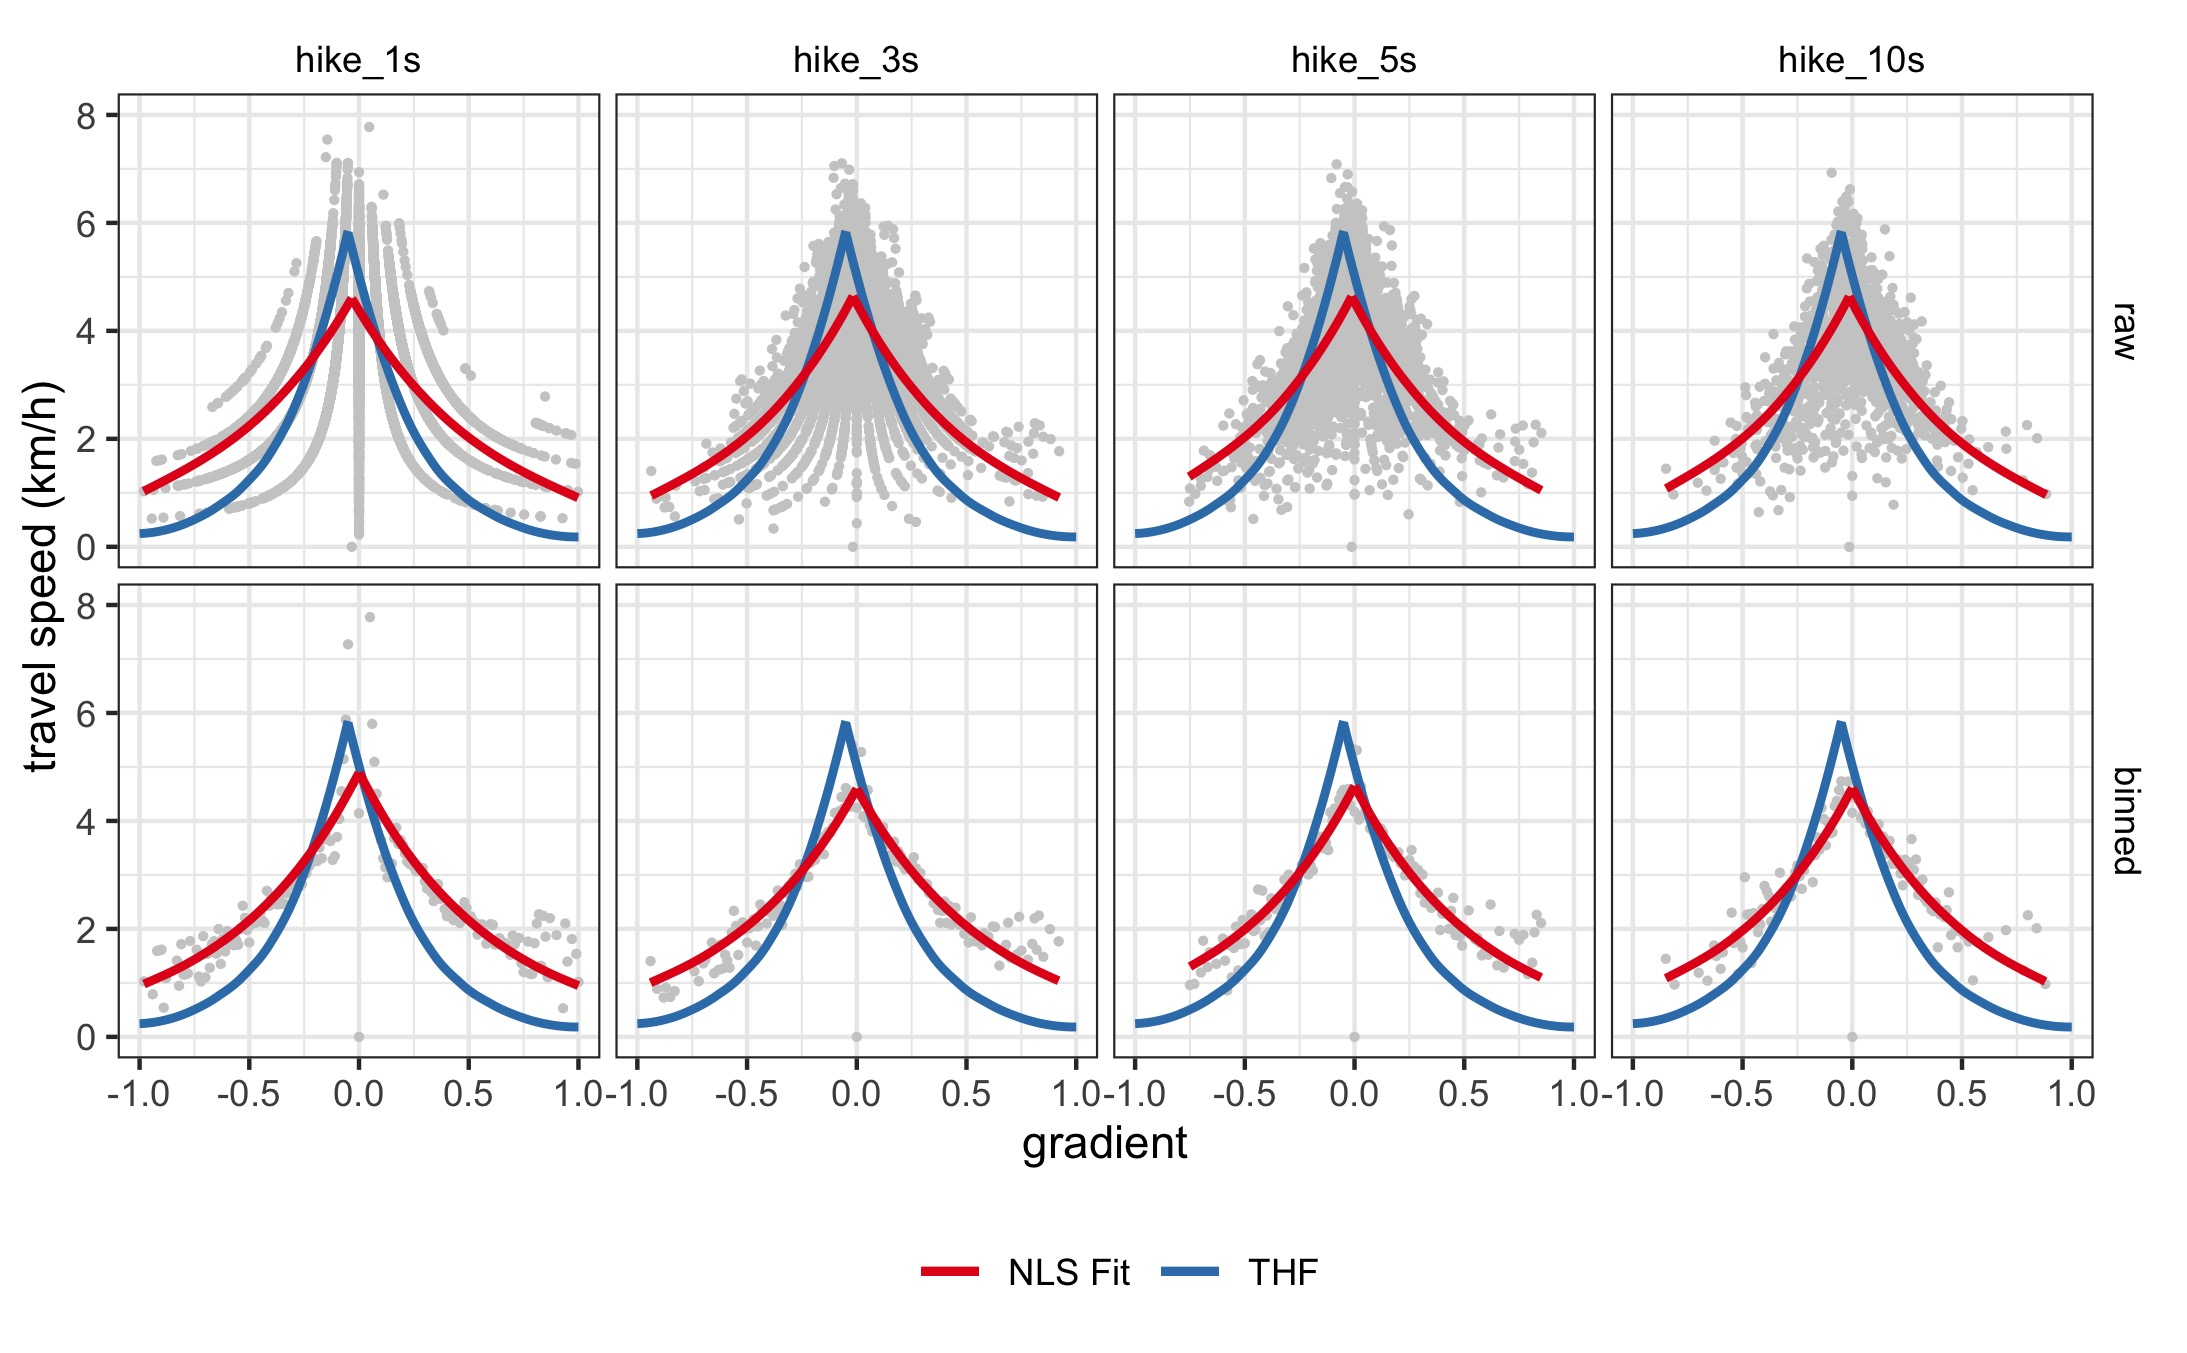
\includegraphics[width=1\linewidth]{./img/Fig_2} \caption{THF and NLS Fit Functions}\label{fig:fig 2}
\end{figure}

Accessibility results for the three travel cost scenarios reveal that
the function fit to my travel performance leads to 2,287 buildings
within a 15 min walk to the Kinwick Centre, which is 1.7\% less than the
number estimated using the original THF. This similarity suggests some
trade-offs are occurring between my lower speeds on flatter ground and
higher speeds on steeper slopes compared to the THF when routing on the
network. For comparison, assuming the network was 2D would result in
2,502 buildings within a 15 min walk which would overestimate my
accessibility by about 9.4\% and 7.6\% compared to the 3D network using
my fit function and the THF respectively. To highlight these
differences, Figure 3 shows 15 min isochrones calculated to the Kinwick
Centre for the three cost scenarios.

While the data uncertainty caveats outlined in Goodchild (2020) apply in
the calibration of the bespoke cost function and propagate to the
accessibility analysis, these findings indicate the strong role of cost
functions in calculating accessibility on 3D networks and the
overestimation of access that can occur when assuming networks are flat.
My results also suggest the potential for the THF to under-estimate
walking speeds on steeper slopes in more urban contexts where stairs are
common. However, while the trails used to calibrate my cost function are
arguably more reflective of urban walking conditions than the unimproved
terrain used to calibrate the original THF, confirming this hypothesis
and increasing confidence in the generalizability of the results will
require further research with a sample size \(n>1\). Nevertheless, the
proliferation of sensors on consumer-grade smart devices and the suite
of movement data they collect offer exciting new opportunities for
calibrating cost functions that can be utilized for accessibility
research and to personalize suggestions for routing on networks rich in
topography.

\begin{figure}[H]
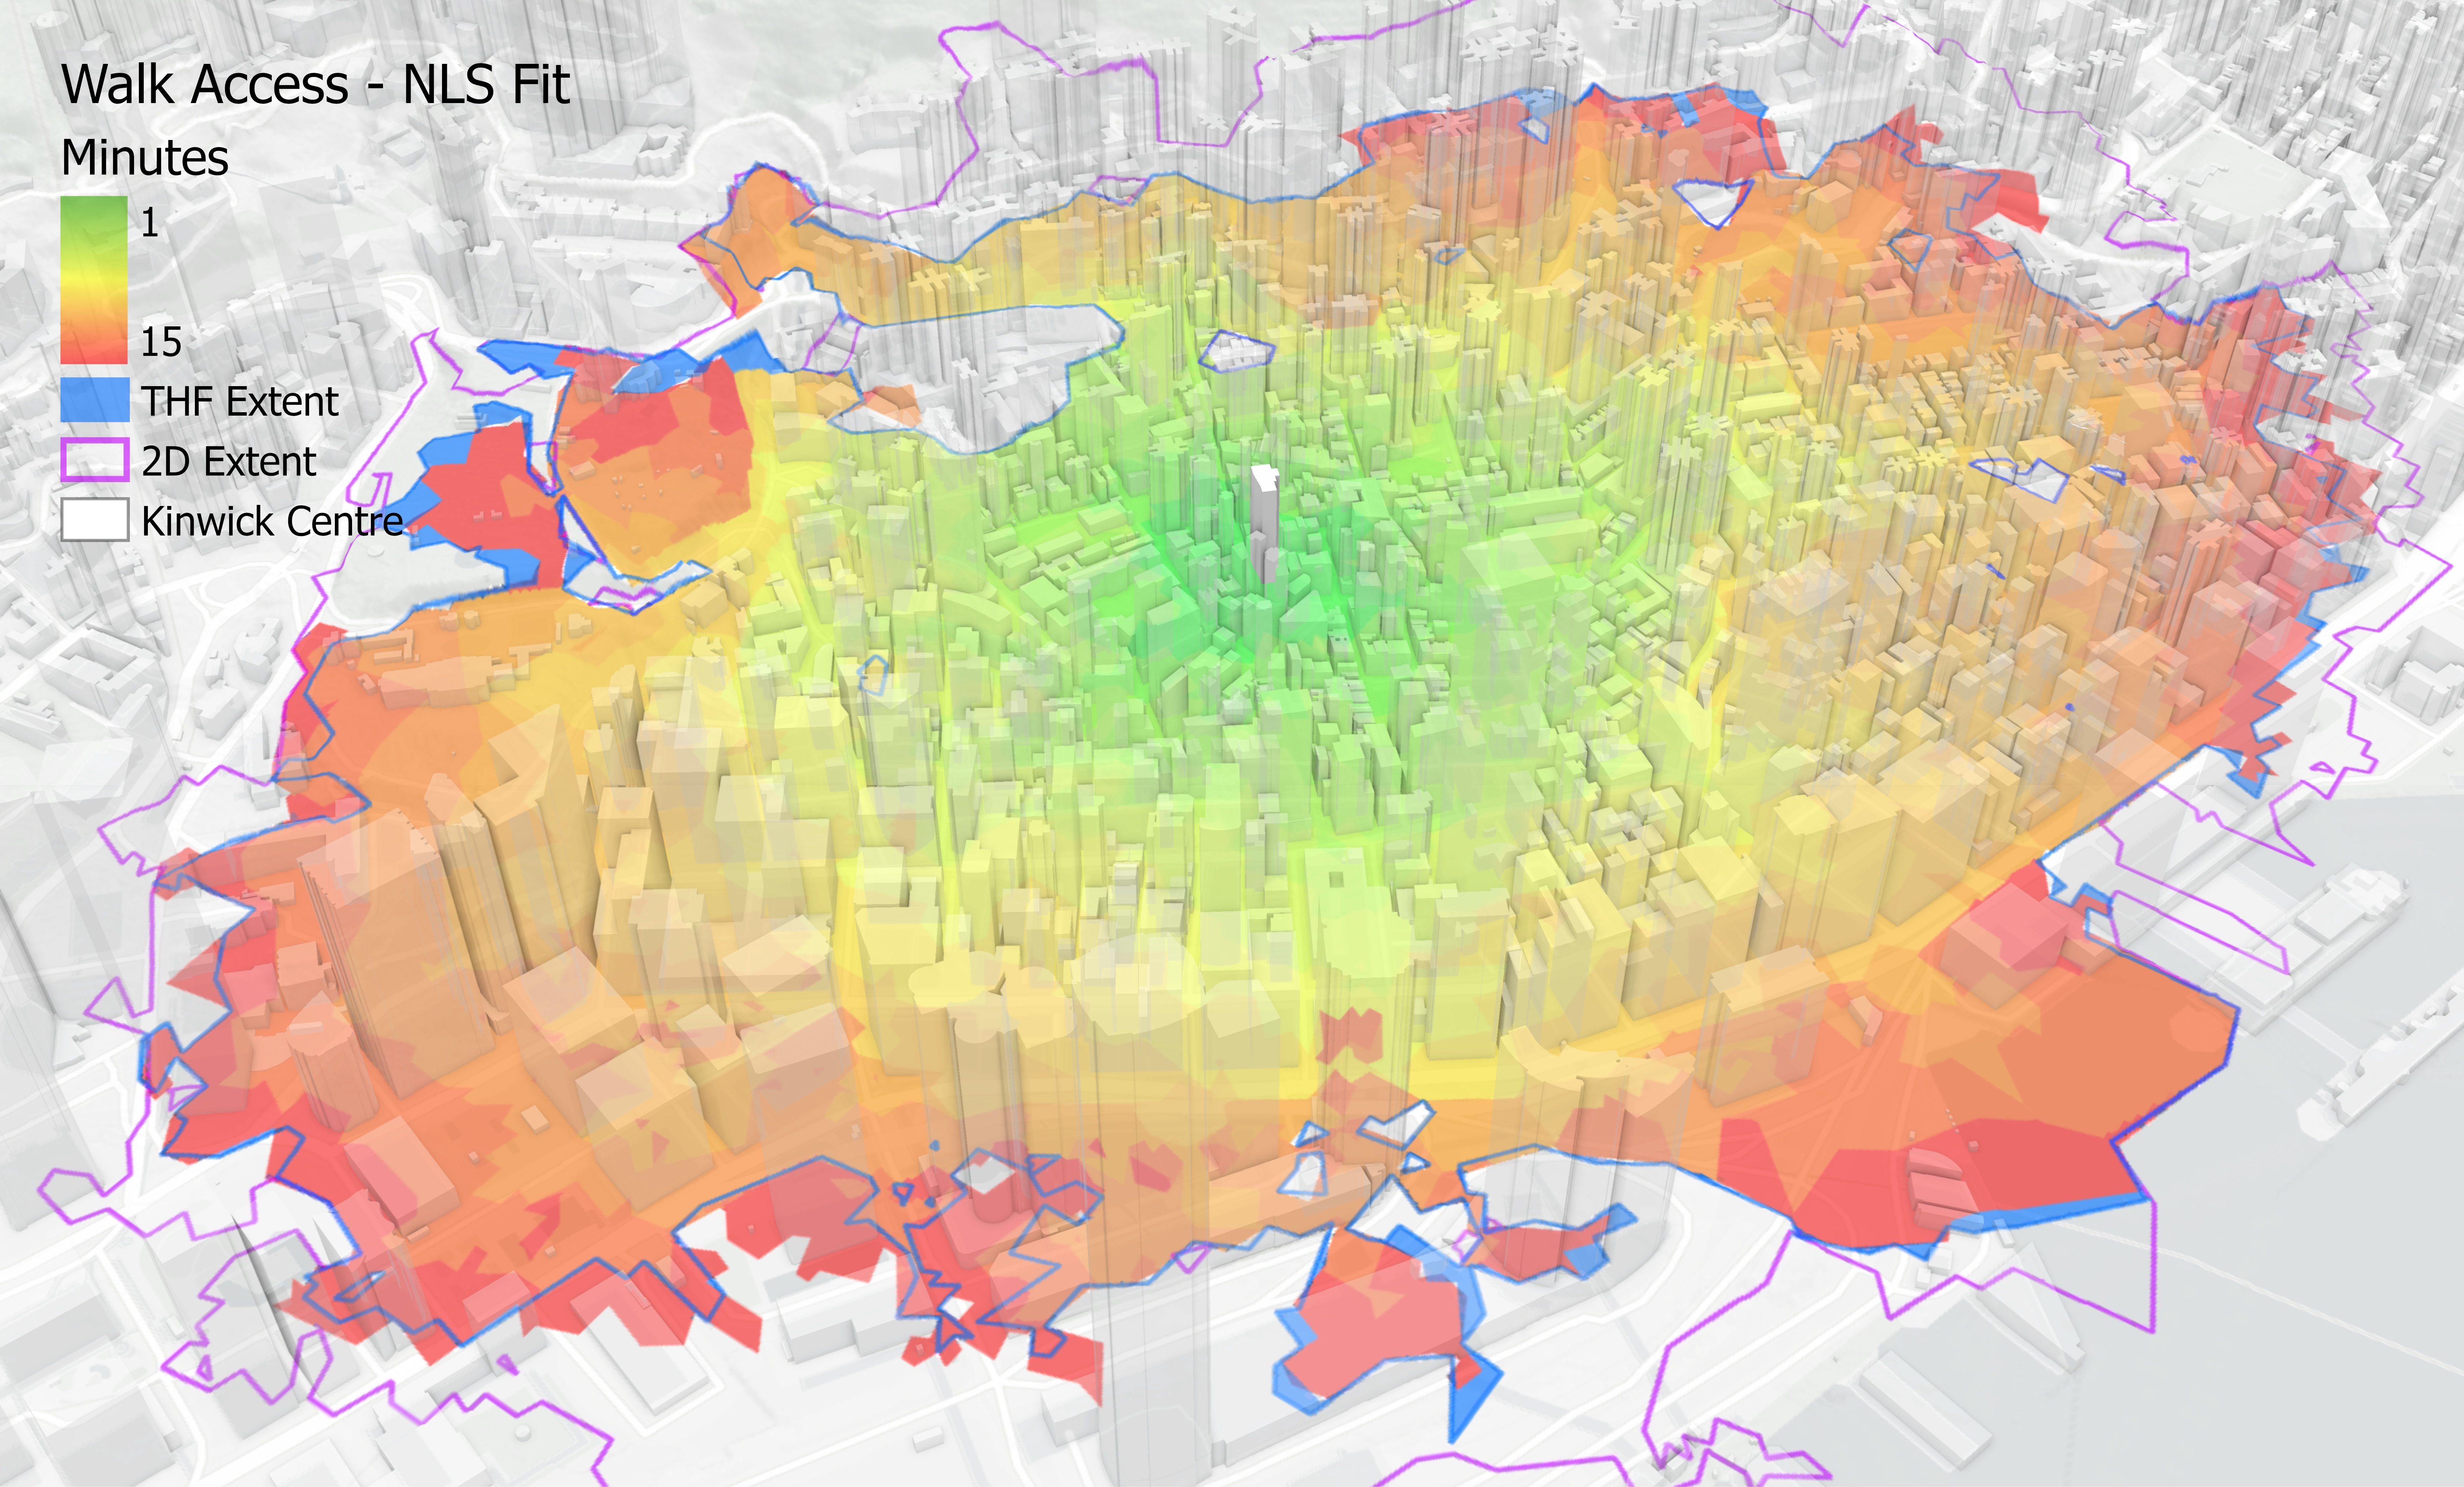
\includegraphics[width=1\linewidth]{./img/Fig_3} \caption{Walk Access Isochrone - NLS Fit Function}\label{fig:fig 3}
\end{figure}

\hypertarget{references}{%
\section*{REFERENCES}\label{references}}
\addcontentsline{toc}{section}{REFERENCES}

\hypertarget{refs}{}
\begin{CSLReferences}{1}{0}
\leavevmode\hypertarget{ref-brundson2018}{}%
Brundson, Chris. 2018. {``Tobler's Hiking Function.''}
\url{https://rpubs.com/chrisbrunsdon/hiking}.

\leavevmode\hypertarget{ref-bruyns2020}{}%
Bruyns, Gerhard JB, Christopher D Higgins, and Darren H Nel. 2020.
{``Urban Volumetrics: From Vertical to Volumetric Urbanisation and Its
Extensions to Empirical Morphological Analysis.''} \emph{Urban Studies}
58 (5): 922--40. \url{https://doi.org/10.1177/0042098020936970}.

\leavevmode\hypertarget{ref-campbell2019}{}%
Campbell, Michael J., Philip E. Dennison, Bret W. Butler, and Wesley G.
Page. 2019. {``Using Crowdsourced Fitness Tracker Data to Model the
Relationship Between Slope and Travel Rates.''} \emph{Applied Geography}
106 (May): 93--107. \url{https://doi.org/10.1016/j.apgeog.2019.03.008}.

\leavevmode\hypertarget{ref-goodchild2020}{}%
Goodchild, Michael F. 2020. {``Beyond Tobler{'}s Hiking Function.''}
\emph{Geographical Analysis} 52 (4): 558--69.
\url{https://doi.org/10.1111/gean.12253}.

\leavevmode\hypertarget{ref-higgins2019}{}%
Higgins, Christopher D. 2019. {``A 4d Spatio-Temporal Approach to
Modelling Land Value Uplift from Rapid Transit in High Density and
Topographically-Rich Cities.''} \emph{Landscape and Urban Planning} 185
(May): 68--82. \url{https://doi.org/10.1016/j.landurbplan.2018.12.011}.

\leavevmode\hypertarget{ref-imhof1950}{}%
Imhof, Eduard. 1950. \emph{Gel{ä}nde Und Karte}. Rentsch.

\leavevmode\hypertarget{ref-irmischer2017}{}%
Irmischer, Ian J., and Keith C. Clarke. 2017. {``Measuring and Modeling
the Speed of Human Navigation.''} \emph{Cartography and Geographic
Information Science} 45 (2): 177--86.
\url{https://doi.org/10.1080/15230406.2017.1292150}.

\leavevmode\hypertarget{ref-ji2010}{}%
Ji, Shengyue, Wu Chen, Xiaoli Ding, Yongqi Chen, Chunmei Zhao, and
Congwei Hu. 2010. {``Potential Benefits of GPS/GLONASS/GALILEO
Integration in an Urban Canyon {{}} Hong Kong.''} \emph{Journal of
Navigation} 63 (4): 681--93.
\url{https://doi.org/10.1017/s0373463310000081}.

\leavevmode\hypertarget{ref-landsd2021}{}%
LandsD. 2021. {``3d Pedestrian Network.''} Lands Department.
\url{https://data.gov.hk/en-data/dataset/hk-landsd-openmap-3d-pedestrian-network}.

\leavevmode\hypertarget{ref-paez2020}{}%
Páez, Antonio, Zoha Anjum, Sarah E. Dickson-Anderson, Corinne J.
Schuster-Wallace, Belén Martín Ramos, and Christopher D. Higgins. 2020.
{``Comparing Distance, Time, and Metabolic Energy Cost Functions for
Walking Accessibility in Infrastructure-Poor Regions.''} \emph{Journal
of Transport Geography} 82 (January): 102564.
\url{https://doi.org/10.1016/j.jtrangeo.2019.102564}.

\leavevmode\hypertarget{ref-pingel2010}{}%
Pingel, Thomas J. 2010. {``Modeling Slope as a Contributor to Route
Selection in Mountainous Areas.''} \emph{Cartography and Geographic
Information Science} 37 (2): 137--48.
\url{https://doi.org/10.1559/152304010791232163}.

\leavevmode\hypertarget{ref-sun2019}{}%
Sun, Guibo, Chris Webster, and Xiaohu Zhang. 2019. {``Connecting the
City: A Three-Dimensional Pedestrian Network of Hong Kong.''}
\emph{Environment and Planning B: Urban Analytics and City Science} 48
(1): 60--75. \url{https://doi.org/10.1177/2399808319847204}.

\leavevmode\hypertarget{ref-tobler1993}{}%
Tobler, Waldo. 1993. {``Non-Isotropic Modeling.''} In \emph{Three
Presentations on Geographical Analysis and Modeling}. {National Center
for Geographic Information and Analysis}.

\end{CSLReferences}

\bibliographystyle{unsrt}
\bibliography{references.bib}


\end{document}
